\section{Theory}

\subsection{How does Augmented Reality work?}

\subsubsection{History of AR}

\subsubsection{S.L.A.M.}

\subsubsection{Depth tracking}

\subsubsection{Cameras}

\subsubsection{Other inputs}
Compass, Gyroscope, Accelerometer  etc.

\subsection{What Machine Learning methods are there?}
There exists many different machine learning techniques out there today. Due to its high effectiveness and relevance, for this report we are going to focus on the highly popular method of neural networks.
This is a proven method for working well with images (Convolutional neural networks) and is therefore a highly 
relevant technique for this project.

\subsubsection{Perceptron}
A perceptron is the simplest form of the neural network. It has a set of inputs and an output.
The perceptron first sums up all the input values, x, multiplied with the weight value, w.
After that it passes that sum through an activation function. This activation function can be everything from a simple f(x)=x to the more complex sigmoid function, depending on the need. More on this in the upcoming section.

\begin{figure}[hbtp]
\begin{center}
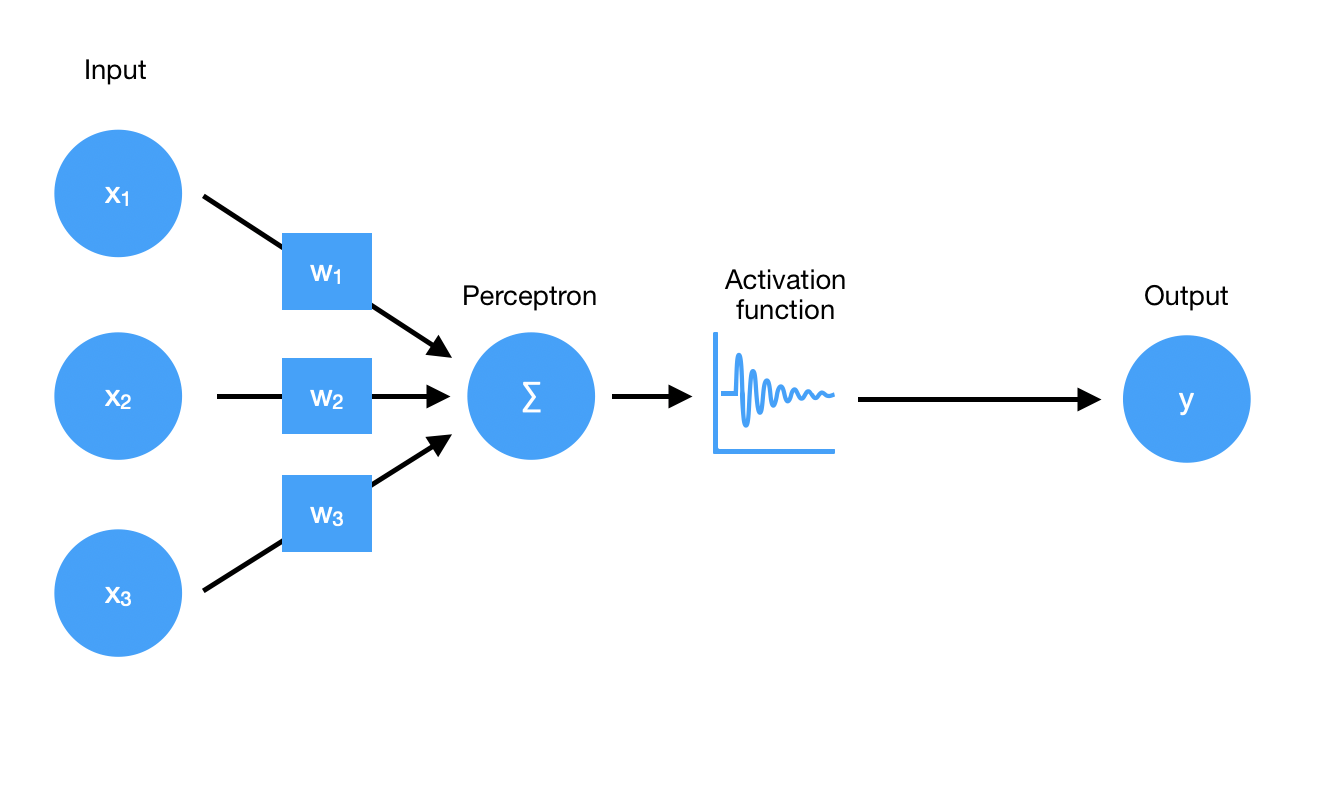
\includegraphics[width = 0.75\textwidth]{./Images/perceptron.jpg} 
\caption{An illustration of the perceptron, the simplest version of a neural network.}
\end{center}
\end{figure}

A bias also exists in every node which is not based on any input. The bias function in the perceptron is similar to what the m in y = kx + m does. It gives the function the ability to move up and down in the graph for more possibilities of splitting the data set. The bias is usually disregarded when illustrating the perceptron.

The perceptron only has the ability to draw a single line and thus is only able to split simple data sets.

*Formula for the output of the perceptron*

\subsubsection{Activation functions}

ReLu
Tanh
Sigmoid

\subsubsection{Loss/Optimizers}

Mean squared

SGD
Adam
Nadam

\subsubsection{Layers}

\begin{figure}[hbtp]
\begin{center}
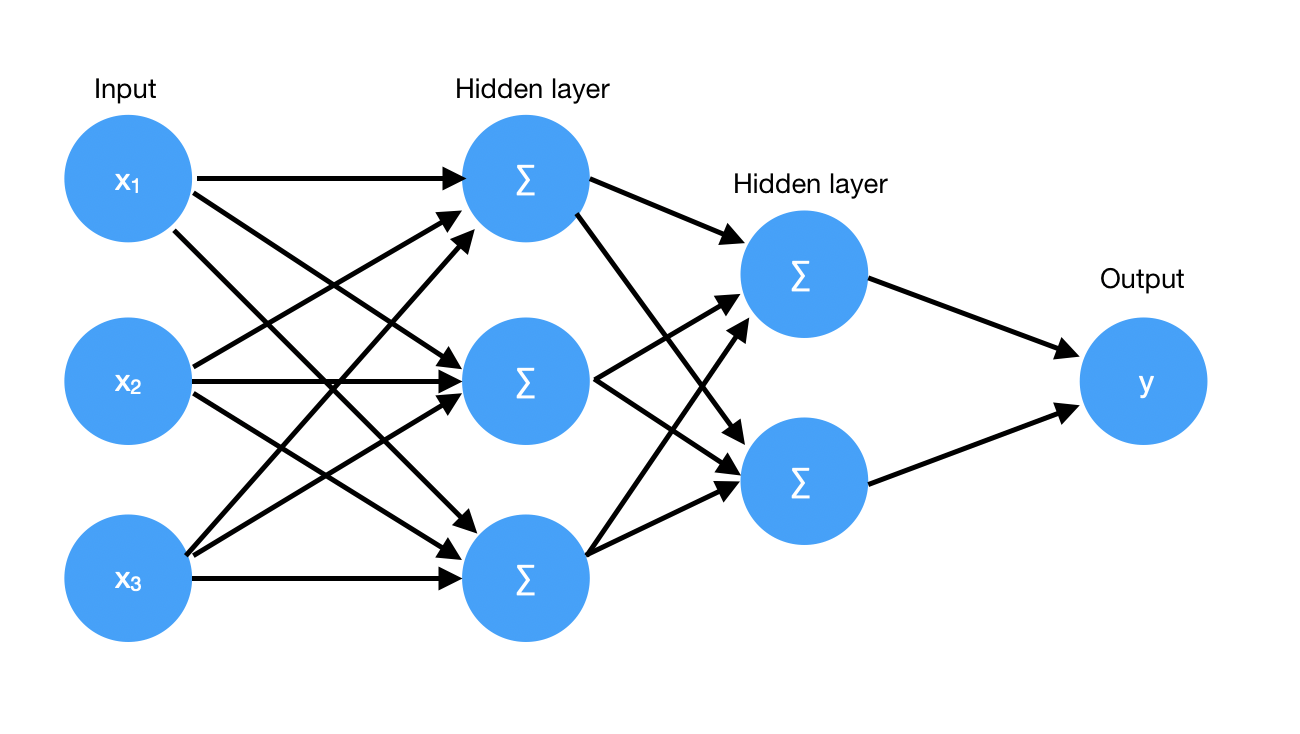
\includegraphics[width = 0.75\textwidth]{./Images/fully_connected.jpg} 
\caption{Two fully connected layers. One with 3 neurons and one with 2 neurons.}
\end{center}
\end{figure}

With more layers and more neurons the networks parameters and complexity begins to grow. So does also the training time, size of the model and the cost for doing predictions. Thus, these networks are capable of describing much more complex data sets. But as a result of that, the risk of overfitting (The act of describing the training data set too well so that new data sets will not get recognized. More on this later.) becomes much greater. That is why a complex network is not always wanted.

\subsubsection{Artificial Neural networks}

\subsubsection{Deep Neural Networks}
% Write about how Deep Neural Networks work and how it's applyed to image classification

\subsubsection{Transfer Learning}
% Write about the theory behind Transfer Learning


\subsection{Object Detection without machine learning}
% Write about feature based detection and segmentation

Foreground/Background segmentation.

There are methods for detecting objects in images. 

Mathematical morphology

Flood fill

Edge detection

Histogram equalisation

One possible way of detecting objects in an image is to use depth data, or RGB-D.
A tool that typically comes to mind when reading about depth data is the Kinect camera
for Xbox.

How depth capture works; True depth, Dual camera depth

The fact that Dual camera depth cannot be captured in real-time in an AR Scene.

Despite all the available methods above, object detection without machine learning is still very tricky. These methods works best when the images are in an controlled environment, typically industrial, like finding screws on a white background.
When the environment is a more casual place tough, like recognizing furnitures indoors, the task becomes much more difficult.

\subsection{Object Detection with machine learning}
% Write about how one can do object detection by the use of ML

\subsubsection{RCNN and its different forms}

\subsubsection{YOLO}

\subsection{Object recognition with machine learning}


\newpage
